% !TEX root = ../VLDB-2026-DAGSmith-Dependency-Aware-Rewriting-for-dbt-Style-SQL-Pipelines.tex
\section{Approach}
\label{sec:approach}

% Required preamble (in main.tex):
%   \usepackage{tikz}
% This file loads its own TikZ libraries below, so no \usetikzlibrary
% is needed in main.tex on its account.

\usetikzlibrary{arrows.meta, positioning, shapes.geometric, fit, calc}

\begin{figure*}[t]
\centering
\resizebox{\textwidth}{!}{%
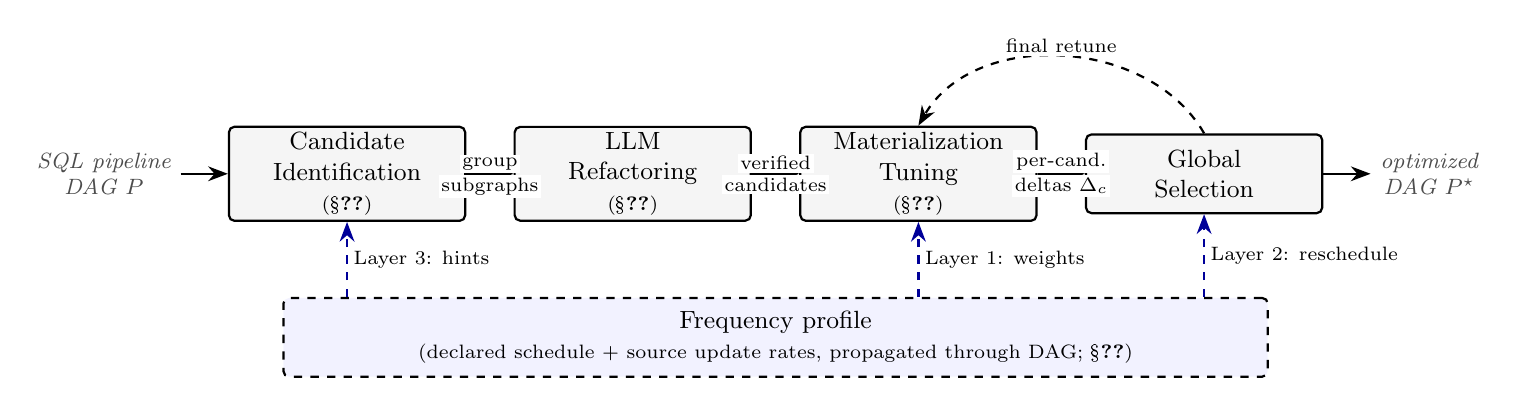
\begin{tikzpicture}[
    font=\small,
    node distance=4mm and 6mm,
    stage/.style={
        draw, rounded corners=2pt, thick,
        minimum height=10mm, minimum width=30mm,
        align=center, fill=black!4,
        inner sep=2pt
    },
    freqstage/.style={
        draw, rounded corners=2pt, thick, dashed,
        minimum height=4mm, minimum width=28mm,
        align=center, fill=blue!5,
        inner sep=2pt
    },
    io/.style={
        align=center, font=\footnotesize\itshape, text=black!70
    },
    arrow/.style={
        -{Stealth[length=2.5mm]}, thick
    },
    freqarrow/.style={
        -{Stealth[length=2.5mm]}, thick, dashed, draw=blue!60!black
    },
    arrowlabel/.style={
        font=\scriptsize, midway, fill=white, inner sep=1pt
    }
]

% --- input ---
\node[io] (input) {SQL pipeline\\DAG $P$};

% --- four pipeline stages, left to right ---
\node[stage, right=of input] (s1) {Candidate\\Identification\\\scriptsize(\S\ref{sec:candidate-identification})};
\node[stage, right=of s1]    (s2) {LLM\\Refactoring\\\scriptsize(\S\ref{sec:llm-refactoring})};
\node[stage, right=of s2]    (s3) {Materialization\\Tuning\\\scriptsize(\S\ref{sec:materialization})};
\node[stage, right=of s3]    (s4) {Global\\Selection};

% --- output ---
\node[io, right=of s4] (output) {optimized\\DAG $P^\star$};

% --- main pipeline arrows with artifact labels ---
\draw[arrow] (input) -- (s1);
\draw[arrow] (s1) -- node[arrowlabel, above]{group} node[arrowlabel, below]{subgraphs} (s2);
\draw[arrow] (s2) -- node[arrowlabel, above]{verified} node[arrowlabel, below]{candidates} (s3);
\draw[arrow] (s3) -- node[arrowlabel, above]{per-cand.} node[arrowlabel, below]{deltas $\Delta_c$} (s4);
\draw[arrow] (s4) -- (output);

% --- frequency profile band: one wide box spanning under stages s1-s4 ---
\node[freqstage, below=2mm of s2.south,
      minimum width=125mm, minimum height=10mm,
      anchor=north] (fband)
  at ($(s1.south west)!0.5!(s4.south east) + (0,-8mm)$)
  {Frequency profile\\\scriptsize(declared schedule + source update rates,
   propagated through DAG; \S\ref{sec:frequency})};

% Frequency arrows: profile feeds the three stages it touches, each labeled by layer
\draw[freqarrow] (fband.north -| s1.south) -- (s1.south)
  node[arrowlabel, right=1pt, fill=white]{\scriptsize Layer 3: hints};
\draw[freqarrow] (fband.north -| s3.south) -- (s3.south)
  node[arrowlabel, right=1pt, fill=white]{\scriptsize Layer 1: weights};
\draw[freqarrow] (fband.north -| s4.south) -- (s4.south)
  node[arrowlabel, right=1pt, fill=white]{\scriptsize Layer 2: reschedule};

% Final tuning loop-back: after selection, retune materialization on combined DAG
\draw[arrow, dashed]
  (s4.north) to[out=120, in=60]
  node[arrowlabel, above, fill=white]{final retune}
  (s3.north);

\end{tikzpicture}%
}
\caption{End-to-end pipeline of \tool. The top row shows the four main stages and the artifacts that flow between them; after global selection, a final materialization pass retunes the combined DAG. The dashed band underneath is the frequency-aware overlay (\S\ref{sec:frequency}): a single frequency profile feeds three of the four stages, contributing structural splitting hints, cost weights for materialization tuning, and schedule corrections at selection.}
\label{fig:pipeline}
\end{figure*}


\linc{Okay in general, I think this section has way too many implementation details and less intuitive lessons. The purpose of a paper is not to document every details of the implementation so that others will recreate every single step. You'll have your code released and they can reference your code anyway. Rather, the purpose is do convery what are the key technical challenges to solve this problem, (intuitively) what are our solutions to solve these challenges and why we choose these solutions, and what lessons did we learn. Implementaiton details are helpful only if we have the space and if that supports our argument for the solution. But having too many can be distracting. I also think having 5 subsections (components) are a bit too many. I would suggest having only 3-4 subsections. (I think earlier you wrote there are 3 optimization dimensions? That might be a good breakdown for the subsections. It seems that in the ablation study you only categorize three optimizations anyway.) And within each subsection, you start with what technical challenges you're going to solve (and why such challenges exist in our problem), and intuitively how your solution works (and why it solves the challenges). A figure illustrating the sollution would be a plus. Then, you go into a little bit of details to just have the audience have a slighly deeper understanding. You can take a look at other papers (or even your previous papers) to see how long this should be. Readers/Reviewers won't appreciate if you add too many details and they couldn't easily get the big picture.}

\tool{} optimizes a SQL pipeline DAG along three interacting dimensions: graph refactoring, materialization, and refresh frequency. \linc{I know Barzan is still reorganizing sections 0-2, but since we have three dimensions here, we know just condense the earlier six opportunites to three, and we have an optimization for each of the opportunity? We can probably connect each of the example in Section 2 to one dimension here as well. Wouldn't this be much more succinct and saving lots of space?} These are the same three dimensions our evaluation ablates, and each corresponds to the opportunities of Section~2: refactoring restructures the DAG to share or remove work (Examples~1 and~2), materialization decides which results are persisted, and frequency aligns each node's execution rate with how often its inputs change (Example~3). They cannot be decided independently. 

% The benefit of a refactoring depends on which nodes are materialized, the best materialization configuration depends on the structure of the DAG, and both depend on how often each node executes. A pipeline with hundreds or thousands of models admits an enormous space of candidate refactorings, materialization assignments, and refresh schedules; exhaustive search is infeasible, and optimizing the three dimensions in separate passes misses these interactions and produces decisions that conflict at the boundaries.

\linc{I think we need to reference Figure 5 at the beginning of this paragraph} \tool{} realizes these dimensions in the pipeline of Figure~\ref{fig:pipeline}. Cheap structural analyses first scan the whole DAG and rank model groups by a fingerprint-based score that estimates the benefit of refactoring them jointly (Section~\ref{sec:candidate-identification}). The top-ranked groups are passed to an LLM, which reasons over each region and proposes one or more concrete refactorings (Section~\ref{sec:llm-refactoring}). 
The structural analyses decide where in the DAG to refactor; the LLM decides what refactoring to perform. \linc{Since we mentioned LLM, I think we need to add one sentence to talk about the correctness guarantee. Otherwise, I think that would be the first question that the reviewer raises.} Every refactoring is adopted only after it passes equivalence checks that the LLM writes for itself and that are tested against the project's real data. A refactoring's benefit depends on how its nodes are materialized, so \tool{} tunes each candidate's materialization with a learned cost model and selects a compatible subset to adopt (Section~\ref{sec:materialization}). The frequency dimension cuts across these stages (Section~\ref{sec:frequency}): it reweights the cost-driven decisions, removes refreshes that recompute unchanged data, and contributes structural splitting candidates to the first stage.





% % Required preamble (add to main.tex if not already there):
% % \usepackage{algorithm}
% % \usepackage{algpseudocode}

% \begin{algorithm}[t]
% \caption{\tool{} optimization pipeline.}
% \label{alg:pipeline}
% \begin{algorithmic}[1]
% \Require SQL pipeline DAG $P$, frequency profile $\Phi$
% \Ensure optimized DAG $P^\star$
% \State $f \gets \textsc{PropagateFrequencies}(P, \Phi)$
% \State $\mathcal{G} \gets \textsc{ReuseAnalysis}(P) \cup \textsc{PruneAnalysis}(P)$
% \Statex \hspace{3.6em} $\cup\ \textsc{FrequencySplitHints}(P, f)$ \Comment{\S\ref{sec:candidate-identification}}
% \State $\mathcal{C} \gets \textsc{LLMRefactor}(\mathcal{G}, P)$ \Comment{\S\ref{sec:llm-refactoring}}
% \State $\delta_{\text{orig}} \gets \textsc{MaterializationTune}(P, f)$ \Comment{\S\ref{sec:materialization}}
% \ForAll{$c \in \mathcal{C}$}
%   \State $P_c \gets \textsc{Apply}(P, c)$
%   \State $\Delta_c \gets \delta_{\text{orig}} - \textsc{MaterializationTune}(P_c, f)$
% \EndFor
% \State $H \gets \textsc{ConflictGraph}(\mathcal{C})$
% \State $\mathcal{C}^\star \gets \textsc{SelectILP}(\mathcal{C}, \{\Delta_c\}, H)$ \Comment{\S\ref{sec:materialization}}
% \State $P^\star \gets \textsc{Apply}(P, \mathcal{C}^\star)$
% \State $\textsc{MaterializationTune}(P^\star, f)$ \Comment{final retune}
% \State \Return $\textsc{ReconcileSchedule}(P^\star, f)$ \Comment{\S\ref{sec:frequency}}
% \end{algorithmic}
% \end{algorithm}


\subsection{Candidate Identification}
\label{sec:candidate-identification}

\linc{I don't think we have established why we want to use LLM for refactoring yet. So I think either you have to establish that here, or just talk about refactoring is costly in general, without specifically emphasizing LLMs.}
Deciding how to refactor a region of the pipeline requires reasoning about what its models compute, a semantic judgment beyond the reach of syntactic rewrite rules, so \tool{} delegates it to an LLM. A project with hundreds of models admits an enormous number of conceivable refactorings, and running the LLM on every model group would be both prohibitively expensive and dominated by trivial proposals. \tool{} therefore divides the labor: cheap structural analyses scan the whole DAG and surface the few regions where a refactoring is likely to pay off, and the expensive LLM reasoning is reserved for those regions.

\linc{Before getting into all the details below, I think it would be good to have one paragraph to discuss intuitively how your analysis works and what it achieves (if you can pair that with a figure, that's even better). The rest of this subsection is just implementation details. If intuitively the method makes sense, we would be good. We can either keep the details below or just condense them if we're short on space.}

At its core the analysis must decide when two models do the same expensive work, and the obvious tests miss real cases. Matching SQL text fails on any rephrasing. Matching plan structure is stronger, since multi-query optimization and view-matching already handle join order, predicate order, and aliasing, but they still miss equivalences that change the plan's shape, and they see only one compiled query at a time. In Figure~\ref{fig:dataflow-grouping}, Models A and B are equivalent but apply a filter on opposite sides of the \textsc{group by}, so a structural matcher sees two different trees. \tool{} instead matches on what each model computes, independent of how the SQL is written and of where the model sits in the DAG, so the two models reduce to one candidate that the LLM and an equivalence check then confirm is safe to share. Two analyses do this: \emph{reuse} finds repeated expensive work to share, and \emph{prune} finds work that no downstream model consumes or that runs too early. Only the highest-scoring regions go to the LLM.
 
\begin{figure}[t]
\centering
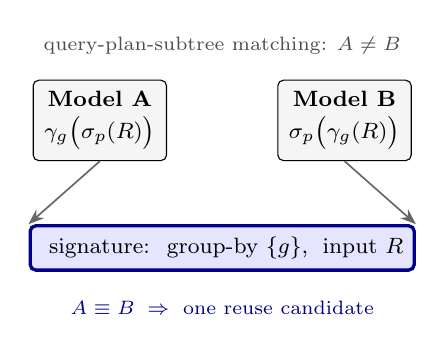
\begin{tikzpicture}[
  font=\small,
  >={Stealth[length=2mm]},
  q/.style={draw, rounded corners=2pt, align=center, fill=black!4, inner sep=4pt, font=\footnotesize},
  canon/.style={draw=blue!55!black, very thick, rounded corners=2pt, align=center, fill=blue!10, inner sep=4pt, font=\footnotesize},
  arr/.style={->, semithick, draw=black!60},
  lbl/.style={font=\scriptsize, text=black!70}
]
\node[q] (A) {\textbf{Model A}\\[2pt]$\gamma_{g}\bigl(\sigma_{p}(R)\bigr)$};
\node[q, right=14mm of A] (B) {\textbf{Model B}\\[2pt]$\sigma_{p}\bigl(\gamma_{g}(R)\bigr)$};
% verdict placed just above the boxes
\node[lbl, anchor=south] (neq) at ($(A.north)!0.5!(B.north)+(0,2mm)$)
  {query-plan-subtree matching: $A \neq B$};
% signature just below the boxes
\node[canon, anchor=north] (C) at ($(A.south)!0.5!(B.south)+(0,-8mm)$)
  {\tool{} signature:\; group-by $\{g\}$,\; input $R$};
\draw[arr] (A.south) -- (C.north west);
\draw[arr] (B.south) -- (C.north east);
\node[lbl, text=blue!55!black, below=2.5mm of C] {$A \equiv B \;\Rightarrow\;$ one reuse candidate};
\end{tikzpicture}
\caption{Candidate identification matches on computation, not on plan shape. Models A and B are equivalent (the filter is on the grouping key) but apply it on opposite sides of the \textsc{group by}, so plan-subtree matching sees two trees, while \tool{} reduces both to one signature and a single reuse candidate.}
\label{fig:dataflow-grouping}
\end{figure}

\head{Dataflow representation}
Both analyses run on a \emph{dataflow representation} that \tool{} builds for each model: its SQL compiled into a tree of typed operators, with every column resolved back through the chain of models that produced it via the project's \texttt{ref()} graph. Models A and B of Figure~\ref{fig:dataflow-grouping} are shown in this form, each applying a filter and a group-by to an input $R$; resolving the columns shows that both group $R$ by the same key $g$, whatever the surrounding SQL looks like and wherever the two models sit in the DAG. The analyses read this representation rather than the SQL text.

\head{Reuse analysis}
Reuse analysis summarizes each model by a signature of its expensive operations (joins and group-by aggregations), their keys, and their resolved inputs, then groups models whose signatures match. A high reuse score is a \emph{targeting signal}, not an instruction to materialize a shared subexpression: it marks where the LLM should look.

\head{Prune analysis}
Prune analysis targets joins, in two forms. A \emph{redundant} join produces a result that no downstream model consumes, confirmed by tracing column lineage from the leaf models; it can be removed outright, and a semi-join collapses to a predicate when its filtering set is already derivable from columns in the probed relation. A \emph{mistimed} join is semantically correct but computed too early: when one side feeds expensive downstream operations whose results do not depend on the other side's columns, pushing the join past those operations avoids carrying its product through them. Prune analysis also flags unused projected columns whose removal simplifies upstream definitions. What sets this apart from local dead-code elimination is its scope: whether a join's result is used, or used too soon, is a fact about the rest of the pipeline that a single-query rewriter cannot see.

\head{From candidates to subgraphs}
The two analyses produce a ranked stream of candidate model groups. For each, \tool{} extracts a subgraph containing the candidate models plus a configurable neighborhood of upstream and downstream context, enough for the LLM to reason about correctness; groups whose neighborhoods exceed the bound are skipped. The next subsection describes how the LLM turns these subgraphs into concrete refactorings.




\subsection{LLM Refactoring}
\label{sec:llm-refactoring}

\linc{Well, why do we want to use an LLM to do this in the first place? We either have to establish this earlier or justify it here.}
As motivated in the overview, producing these cross-boundary, semantic rewrites is a reasoning task rather than a pattern-matching one, which is why \tool{} uses an LLM rather than a fixed rule set. But asking an LLM to rewrite SQL that will run against a production warehouse raises three problems: the rewrite may be \emph{slower} than the original, may be \emph{incorrect}, or may be \emph{too expensive to generate} when a region contains many models. The challenge for this stage is to obtain useful rewrites while controlling all three risks.

\linc{Similarly, I think one paragraph to discuss intuitively how your approach works and what it achieves (better with a figure) can be valuable. The details can be reduce.}
\tool{} controls these risks by refusing to treat rewriting as a single LLM call. It splits the work into four roles, each a separate call with one job: a \emph{proposer} reads the region and lists candidate optimizations, an adversarial \emph{critic} rejects proposals that would slow the pipeline or silently change its results, a \emph{rewriter} turns the survivors into concrete SQL, and a \emph{verifier} tests each rewrite against the warehouse's real data before it is trusted. Separating proposal from criticism keeps a single prompt from having to be both creative and skeptical, and grounding acceptance in real data rather than in the model's own assurance is what makes adopting LLM-written SQL safe. A fifth, lighter mechanism propagates an accepted rewrite across near-duplicate models, so the four-call sequence need not run on each one.

\head{Proposal}
The first call ingests the subgraph's SQL and dependency edges and produces a domain-level reading of the region: a short semantic summary of each model and the end-to-end business question the subgraph answers. This reading is what lets later stages recognize equivalent computations written in dissimilar SQL. Its output is a list of \emph{opportunities}, each naming the work it would remove or shrink and the mechanism by which it would do so; opportunities are proposals, not yet rewrites.

\head{Filtering}
A second call acts as an adversarial critic over the proposals. The separation is deliberate: a single LLM asked at once to propose and to doubt does neither well, with proposal mode dominating. The critic catches both slowdowns and correctness traps. A slowdown is, for instance, a proposal that looks like reuse-driven savings but adds a write and a scan without reducing downstream work. A correctness trap is shown in Figure~\ref{fig:critic-catch}: the proposal drops a join by reading a tag from a sibling that has been deduplicated to one row per item, silently discarding the secondary tags the original join admitted. The critic returns one of three verdicts, \emph{approve}, \emph{reject}, or \emph{conditional}; a conditional verdict records a data property the rewrite must hold to, which is carried into the next stage.

\begin{figure}[!htbp]
\begin{minipage}[t]{0.48\linewidth}
\figsubheader{Original: join admits all tags}
\begin{lstlisting}[language=SQL]
SELECT i.item_id,
  MAX(CASE WHEN t.tag='A'
    THEN 1 ELSE 0 END) AS flag_a
FROM {{ ref('items') }} i
JOIN {{ ref('item_tags') }} t
  USING (item_id)
GROUP BY i.item_id
\end{lstlisting}
\end{minipage}
\hfill
\begin{minipage}[t]{0.48\linewidth}
\figsubheader{Proposal: drop join, read tag}
\begin{lstlisting}[language=SQL]
SELECT s.item_id,
  CASE WHEN s.tag='A'
    THEN 1 ELSE 0 END AS flag_a
FROM {{ ref('items_staged') }} s
-- items_staged keeps one tag/item;
-- secondary tags are silently lost
\end{lstlisting}
\end{minipage}
\caption{Correctness trap rejected by the proposal critic. The original aggregates over all tags per item; the proposal reads from a sibling that has been deduplicated to one tag per item, and silently drops the rest.}
\label{fig:critic-catch}
\end{figure}

\head{Rewriting}
The opportunities that survive filtering, together with the analysis and the SQL of the affected nodes, go to a third call that produces concrete refactored SQL: it may rewrite nodes, mark nodes as removed, or introduce new shared nodes. Conditional opportunities carry their recorded constraints into this prompt. A node with consumers outside the subgraph may be rewritten internally but must produce identical output rows, since its contract with those consumers is fixed.

\head{Equivalence verification}
A rewrite that passed filtering can still change the data, especially when one bundles several opportunities and a trap rejected on its own reappears nested inside a larger change: the staged-input shortcut of Figure~\ref{fig:critic-catch}, for instance, can resurface inside a consolidated aggregation the critic approved on other grounds. \tool{} therefore treats equivalence as an empirical question against real data. A fourth call, the \emph{correctness critic}, states for each adopted opportunity the data invariant that must hold for the rewrite to be safe and renders it as a SQL diagnostic that returns zero rows when the invariant holds and rows when it is violated. The diagnostics run against the target warehouse under a per-query byte cap; any returned row is a counterexample drawn from real data. Failed invariants are appended to the rewriting prompt, and the LLM must either find a distinctly different strategy that respects them or restore the original logic. The loop ends when the rewrite passes all diagnostics, the LLM reports no further distinct strategy, or a per-group attempt budget is exhausted, in which case the group reverts to its original SQL and contributes no candidate.

\head{Model families and propagation}
A single subgraph often contains many near-duplicate models that apply the same operation to different data subsets. The proposal stage identifies such a group, designates one \emph{representative}, and records how the other members differ; only the representative runs through the four calls above, after which a lighter per-member call applies the same change in parallel. This is a scalability mechanism for projects whose models exhibit family structure; where there is none, the family map collapses to singletons and the main sequence simply runs over every model.


\subsection{Materialization Tuning}
\label{sec:materialization}

A refactoring has no benefit that can be read off in isolation. Whether it helps depends on which of its nodes are stored as tables and which are inlined as views, the best choice differs from one candidate to the next, and the choice is non-local: inlining one node changes the predicted cost of every node downstream of it. \tool{} therefore scores every candidate under its own best materialization assignment, with the unrefactored DAG included as a candidate and serving as the baseline. A second challenge arises once the candidates are scored: they overlap, so two refactorings can touch the same model and cannot both be adopted, and the chosen ones must be composed into a single project rather than taken all at once. This subsection covers both, finding a candidate's best materialization and then selecting a compatible set.

\head{Cost of a DAG configuration}
Given a materialization assignment, the pipeline's cost is computed in one topological pass. A table pays its own predicted slot time once per execution and exposes its predicted cardinality to its children; a view pays no slot time of its own and instead pushes its SQL features and its parents' cardinality forward into every node that reads it, scaled by how often it is referenced. Each node is therefore scored not on the raw counts from its own SQL but on a vector that has accumulated the contributions of every view in its upstream chain, so flipping a single node between table and view changes the predicted cost of all its descendants.

\head{Cost model}
Two Huber regression models, trained on instrumented runs of the original pipeline, supply the per-node predictions the pass consumes: one for a table's cardinality and one for its slot time, each from SQL features parsed out of the compiled query (join and predicate structure, group-by and distinct operations, unions, and table scans, plus window functions and aggregations for slot time). Both predictions are conditioned on the cardinality of the node's parents under the current assignment, and both training and prediction operate on the view-expanded vectors above, so the model sees, for each node, exactly the work it would perform in the configuration being scored. Huber loss is used in place of squared error to limit the pull of a few very large queries.

\head{Iterative local linearization}
Minimizing the total cost over the materialization vector \(t \in \{0,1\}^{|V|}\) is a discrete non-linear problem whose interactions run through every view chain in the DAG, and it is intractable at realistic size. \tool{} applies iterative local linearization, a standard successive-approximation scheme for discrete non-linearities: linearize the cost around the current configuration, solve the linear surrogate, move, and repeat until the configuration stops changing. The result is a locally consistent assignment rather than a global optimum, which is the practical price of feasibility.

Concretely, at iteration \(k\), holding the current assignment \(t^{(k)}\) fixed, \tool{} uses the cost model to measure two local quantities: a baseline build cost \(B^{(k)}_j\) for each node \(j\) (its direct parents forced to tables) and an edge-local delta \(U^{(k)}_{ij}\), the extra cost at \(j\) when only parent \(i\) is inlined as a view. Treating these as constants for the iteration, it solves a small ILP for \(t^{(k+1)}\):
\begin{equation*}
\min_{t,\,y}\; \sum_{j \in V} t_j\, B^{(k)}_j \;+\; \sum_{i \to j \in E} y_{ij}\, U^{(k)}_{ij}, \qquad \text{s.t.}\quad y_{ij} = (1 - t_i) \wedge t_j,
\end{equation*}
where the auxiliary \(y_{ij} \in [0,1]\) is \(1\) exactly when \(j\) executes and reads from a parent \(i\) inlined as a view (linearized by \(y_{ij} \le 1 - t_i\), \(y_{ij} \le t_j\), \(y_{ij} \ge t_j - t_i\), \(y_{ij} \ge 0\)). A node thus pays \(B^{(k)}_j\) when it is a table and an additional \(U^{(k)}_{ij}\) for each view parent. A trust-region cap on flips per iteration and a small flip penalty keep each step inside the region where the local coefficients remain valid; \(B\) and \(U\) are recomputed after a move, since flipping a node changes the cardinalities its descendants see. The loop terminates on convergence, on a repeated assignment, or at an iteration cap. Two pieces of domain knowledge steady the search: nodes with many descendants are pinned as tables, since inlining them recomputes their work for every consumer, and seed and source tables stay tables throughout, since their materialization is not under the project's control.

\head{From a candidate to a delta}
For the original project every model has a measured cardinality and slot time, and the loop runs directly. A refactored candidate has new models with no measurements; its compiled manifest is fed through the same pass, with the cost model predicting each new model's cardinality from its features and its parents', after which the candidate is handled exactly like the original. The candidate's \emph{delta} is the cost of the original under its own best materialization minus the cost of the candidate under its own: the predicted cost reduction the refactoring delivers when adopted in isolation.

\head{Global selection}
These deltas are each measured as if the candidate were adopted alone, but the candidates cannot simply be unioned. Two groups \emph{conflict} when they rewrite, create, or remove any of the same models, since merging two independent rewrites of one model is something no stage has produced or verified; and within a group the LLM may offer several variants of one opportunity, of which at most one is adoptable. \tool{} builds a conflict graph by intersecting the changed-model sets of every pair of groups, then solves a small ILP that maximizes the total adopted delta under two constraints: at most one variant per group, and no two conflicting groups together. The problem is sparse (one binary per candidate and per group) and an off-the-shelf MILP solver dispatches it exactly. Because each delta was measured under the candidate's own isolated materialization, the tuning above is run once more on the combined project, since the optimal assignment for the chosen combination need not coincide with any one candidate's.


\subsection{Frequency-Aware Optimization}
\label{sec:frequency}

The stages so far treated each node's slot time as a fixed per-execution cost. In a recurring SQL pipeline that is wrong in a way that matters: different sources update at different rates, different consumers require fresh output at different rates, and a node's real contribution is its per-run cost multiplied by how often it must actually run. Treating cost as per-execution overvalues savings on rarely-run models, undervalues them on frequently-run ones, and hides a class of refactoring entirely. \tool{} therefore adds a frequency dimension that enters at three layers. Frequencies are taken from the declared schedule at sink nodes and observed update rates at source tables and propagated through the interior of the DAG. Layers 1 and 2 reweight and reschedule the existing DAG without changing its structure; layer 3 feeds a new class of structural candidates back to candidate identification (Section~\ref{sec:candidate-identification}).

\head{Layer 1: Frequency as cost weight}
Materialization tuning and candidate selection (Section~\ref{sec:materialization}) both minimize cost as if every model executed at the same rate. Replacing per-execution slot time with frequency-weighted slot time changes the answer: a refactoring that saves work on a daily-refresh model is worth more than the same per-execution saving on a weekly one. The local coefficients of the linearization are scaled before the ILP runs,
\begin{equation*}
B^{(k)}_j \leftarrow f_j \cdot B^{(k)}_j, \qquad U^{(k)}_{ij} \leftarrow f_j \cdot U^{(k)}_{ij},
\end{equation*}
where \(f_j\) is node \(j\)'s effective frequency, and the selection ILP inherits the same reweighting through the deltas it consumes.

\head{Layer 2: Reconciling scheduled and effective frequency}
A model's effective frequency is the rate at which its schedule fires \emph{and} produces new output, not the rate at which it fires. Each model has a \emph{demand} frequency \(f_j^{\text{demand}}\), set by the rate at which its consumers need fresh output, and a \emph{data-changing} frequency \(f_j^{\text{data}}\), set by the rate at which any of its inputs actually change; the rate at which it contributes useful work is
\begin{equation*}
f_j = \min\!\left(f_j^{\text{demand}},\, f_j^{\text{data}}\right).
\end{equation*}
Where the scheduled rate exceeds \(f_j\), the model is over-scheduled: it executes, reads its inputs, and produces output identical to last time. \tool{} flags such models and reduces their schedule to \(f_j\). This changes no SQL and no materialization, only the schedule, but the saving is immediate, since every redundant execution is eliminated outright. The same \(f_j\) is the weight Layer 1 uses, so the two layers compose.

\head{Layer 3: Frequency-driven splitting hints}
The first two layers leave the DAG structure intact. The third generates structural candidates that the dataflow analyses of Section~\ref{sec:candidate-identification} cannot find on shape alone. When a model has parents with different data-changing frequencies it inherits the fastest one, so any work inside it that depends only on slow-changing parents is re-executed at the fast rate even though its inputs have not changed. \tool{} identifies models whose parent frequencies are heterogeneous and whose slow-side computation is non-trivial and emits the location to candidate identification as a hint, alongside the reuse and prune signals. The hint enters the LLM stage in the same form as any other candidate region, and the LLM proposes a frequency-split refactoring of the kind illustrated in motivating Example~3: the slow-side computation is extracted into a separate model that runs on the slow cadence, and the original becomes a lightweight join over its output. From there the candidate flows through the same filtering, rewriting, verification, scoring, and selection stages as any other, with Layers 1 and 2 active throughout.